\documentclass[12pt]{article}

\usepackage[a4paper,margin=2.5cm,footskip=0.7cm,headheight=1cm]{geometry}

\usepackage{mathtools}
\usepackage{amsmath}
\usepackage{scalerel,amssymb}
\usepackage{gensymb}
\usepackage{graphicx}
\usepackage{caption}
\usepackage{german}
\usepackage{tikz}

\newcommand{\overtext}[2]{\mathrel{\overset{\makebox[0pt]{\mbox{\normalfont\tiny\sffamily #2}}}{#1}}}
\newcommand{\comment}[1]{}
\DeclarePairedDelimiter\abs{\lvert}{\rvert}
\DeclarePairedDelimiter\brackets{(}{)}

%TODO
\title{\vspace{-2.0cm}Aufgabe 1}
\author{Nikolas Kilian}
\date{8. März 2019}

\usepackage{Csharp}
\usepackage{lastpage}
\usepackage{fancyhdr}
\pagestyle{fancy} 

\makeatletter
\let\runauthor\@author
\makeatother
\lhead{\runauthor}
\cfoot{\thepage\ von \pageref{LastPage}}

\begin{document}
\maketitle

\section{Lösungsidee}
Wenn es keine Hindernisse gibt, so ist der optimale Weg eine gerade Strecke vom Startpunkt zum Buspfad im 30\degree\ Winkel. Für Begründung davon siehe 1.1.\\
Gibt es Hindernisse, so ist der optimale Weg der optimale Weg zu einem Eckpunkt, von dem die 30\degree\ Strecke offen ist, und dann diese 30\degree\ Strecke.\\
Um das Optimum mit Hindernissen zu finden, muss man also alle Eckpunkte bestimmen, von denen aus diese 30\degree\ Strecke offen ist, und den optimalen Weg zu ihnen bestimmen. Da der optimale Weg das Format der resultierenden Wege hat, ist unter den resultierenden Wegen das Optimum enthalten, also muss man nun nur noch die Zeit, zu der Lisa loslaufen muss, für alle Wege errechnen und den Weg mit der spätesten Startzeit auswählen.
Der optimale Weg zu diesen Eckpunkten lässt sich bestimmen mithilfe eines Sichtbarkeitsgraphen und Dijkstra's Algorithmus. Zum verhindern von Strecken durch unendlich dünne Wege (berührende Polygone) veränderet man den Sichtbarkeitsgraphen, sodass für jede normal sichtbare Linie nachträglich auf unendlich dünne Wege geprüft werden.

\subsection{Berechnung}
\newcommand{\vb}{v_{Bus}}
\newcommand{\vl}{v_{Lisa}}

\newcommand{\x}{x}

\renewcommand{\a}{a}
\renewcommand{\b}{b}
\renewcommand{\c}{c}

\newcommand{\f}{f}

\newcommand{\tf}{t(\f)}
\newcommand{\df}[1]{\frac{d#1}{d\f}}
\newcommand{\dtf}{\df{\tf}}

\begin{minipage}{0.8\textwidth}
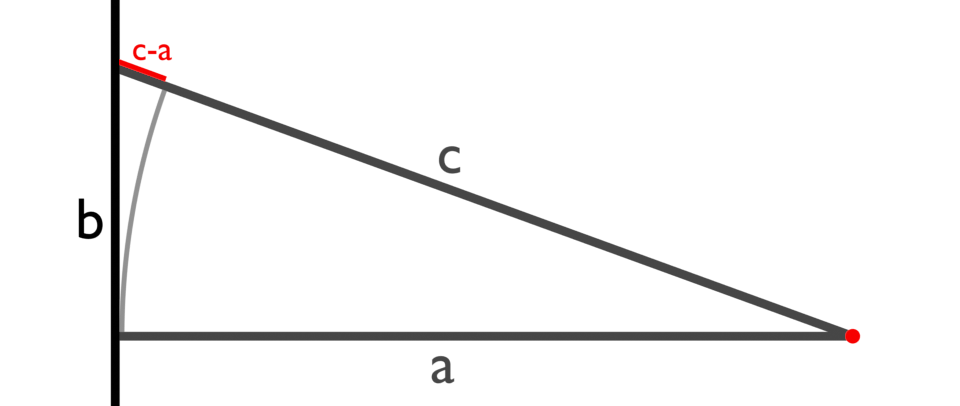
\includegraphics[scale=0.4]{CalcLabel}
\end{minipage}
\begin{minipage}{0.15\textwidth}
\vspace{-1cm}
\[\c=\sqrt{\a^2+\b^2}\]
\[\f:=\frac{\b}{\a}\]%\b=\a\f\]
\end{minipage}

\begin{minipage}{0.45\textwidth}
\begin{align*}
\tf &= \frac{\c-\a}{\vl} - \frac{\b}{\vb}\\
&= \frac{\sqrt{\a^2+\b^2}-\a}{\vl} - \frac{\a\f}{\vb}\\
&= \frac{\sqrt{\a^2(1+\f^2)}-\a}{\vl} - \frac{\a\f}{\vb}\\
&= \a\left(\frac{\sqrt{1+\f^2}-1}{\vl} - \frac{\f}{\vb}\right)\\
\end{align*}
\end{minipage}
\begin{minipage}{0.55\textwidth}
\begin{align*}
\dtf &= \df{\a\left(\frac{\sqrt{1+\f^2}-1}{\vl} - \frac{\f}{\vb}\right)}\\
&= \a\left(\df{\frac{\sqrt{1+\f^2}-1}{\vl}} - \df{\frac{\f}{\vb}}\right)\\
&= \a\left(\frac{\df{\sqrt{1+\f^2}}}{\vl} - \frac{\df{\f}}{\vb}\right)\\
&= \a\left(\frac{\frac{1}{2\sqrt{1+\f^2}}\cdot\df{1+\f^2}}{\vl} - \frac{1}{\vb}\right)\\
&= \a\left(\frac{f}{\vl\sqrt{1+\f^2}} - \frac{1}{\vb}\right)\\
\end{align*}
\end{minipage}

\begin{align*}
&&\dtf &= 0\\
\iff&&\a\left(\frac{f}{\vl\sqrt{1+\f^2}} - \frac{1}{\vb}\right) &= 0\\
\iff&&\a\frac{f}{\vl\sqrt{1+\f^2}} &= \a\frac{1}{\vb}\\
\iff&&\frac{f}{\sqrt{1+\f^2}} &= \frac{\vl}{\vb}\\
\iff&&\left(\frac{f}{\sqrt{1+\f^2}}\right)^2 &= \left(\frac{\vl}{\vb}\right)^2\\
\iff&&\frac{f^2}{1+\f^2} &= \frac{\vl^2}{\vb^2}\\
\iff&&\frac{1+\f^2}{f^2} &= \frac{\vb^2}{\vl^2}\\
\iff&&\frac{1}{f^2} &= \frac{\vb^2-\vl^2}{\vl^2}\\
\iff&&f^2 &= \frac{\vl^2}{\vb^2-\vl^2}\\
\iff&&f &= \sqrt{\frac{\vl^2}{\vb^2-\vl^2}}\\
\iff&&f &= \frac{\vl}{\sqrt{\vb^2-\vl^2}}\\
\end{align*}

\section{Umsetzung}
Zur Umsetzung habe ich mich für eine Implementation in C\# entschieden, mit einer Visualisierung mithilfe von WPF.
Für die Generierung von Sichtbarkeitspolygonen verwende ich eine Implementation des Sweep-Line Algorithmus [Sources here]. Die Version des Algorithmus die ich verwende funktioniert wie folgt:
\begin{Csharp}
Let Intersections = Binary Search Tree, sorted by the order of intersection

foreach (Point p in Points sorted by their angle to Origin) {
	Intersections.RemoveAll(Connected Edges on Clockwise Side of p); 
	
	if (IsVisible(p)) VisibleVertices.Add(p);	
	
	Intersections.AddAll(Connected Edges on Counterclockwise Side of p);
}

boolean IsVisible(p) {
    if (!Origin.BetweenNeighbours(p) || !p.BetweenNeighbours(Origin)) return false;
    if (Origin and p are neighbours) return true;

    if (Intersections is not empty and its leftmost element intersects the line from Origin to Target) return false;
}
\end{Csharp}

\begin{minipage}{0.6\textwidth}
P.BetweenNeighbours(A) gibt dabei zurück, ob für einen Punkt P der Teil eines Polygons ist ob A in dem in Abb. 1 grün markiertem Bereich liegt. Ist das Polygon in P konvex, so ist das Ergebnis immer false.

Wenn der Rückgabewert dieser Methode false ist, so sind in einem reduziertem Sichtbarkeitsgraph die beiden Punkte nicht verbunden.
\end{minipage}\hspace{0.5cm}
\begin{minipage}{0.35\textwidth}
\frame{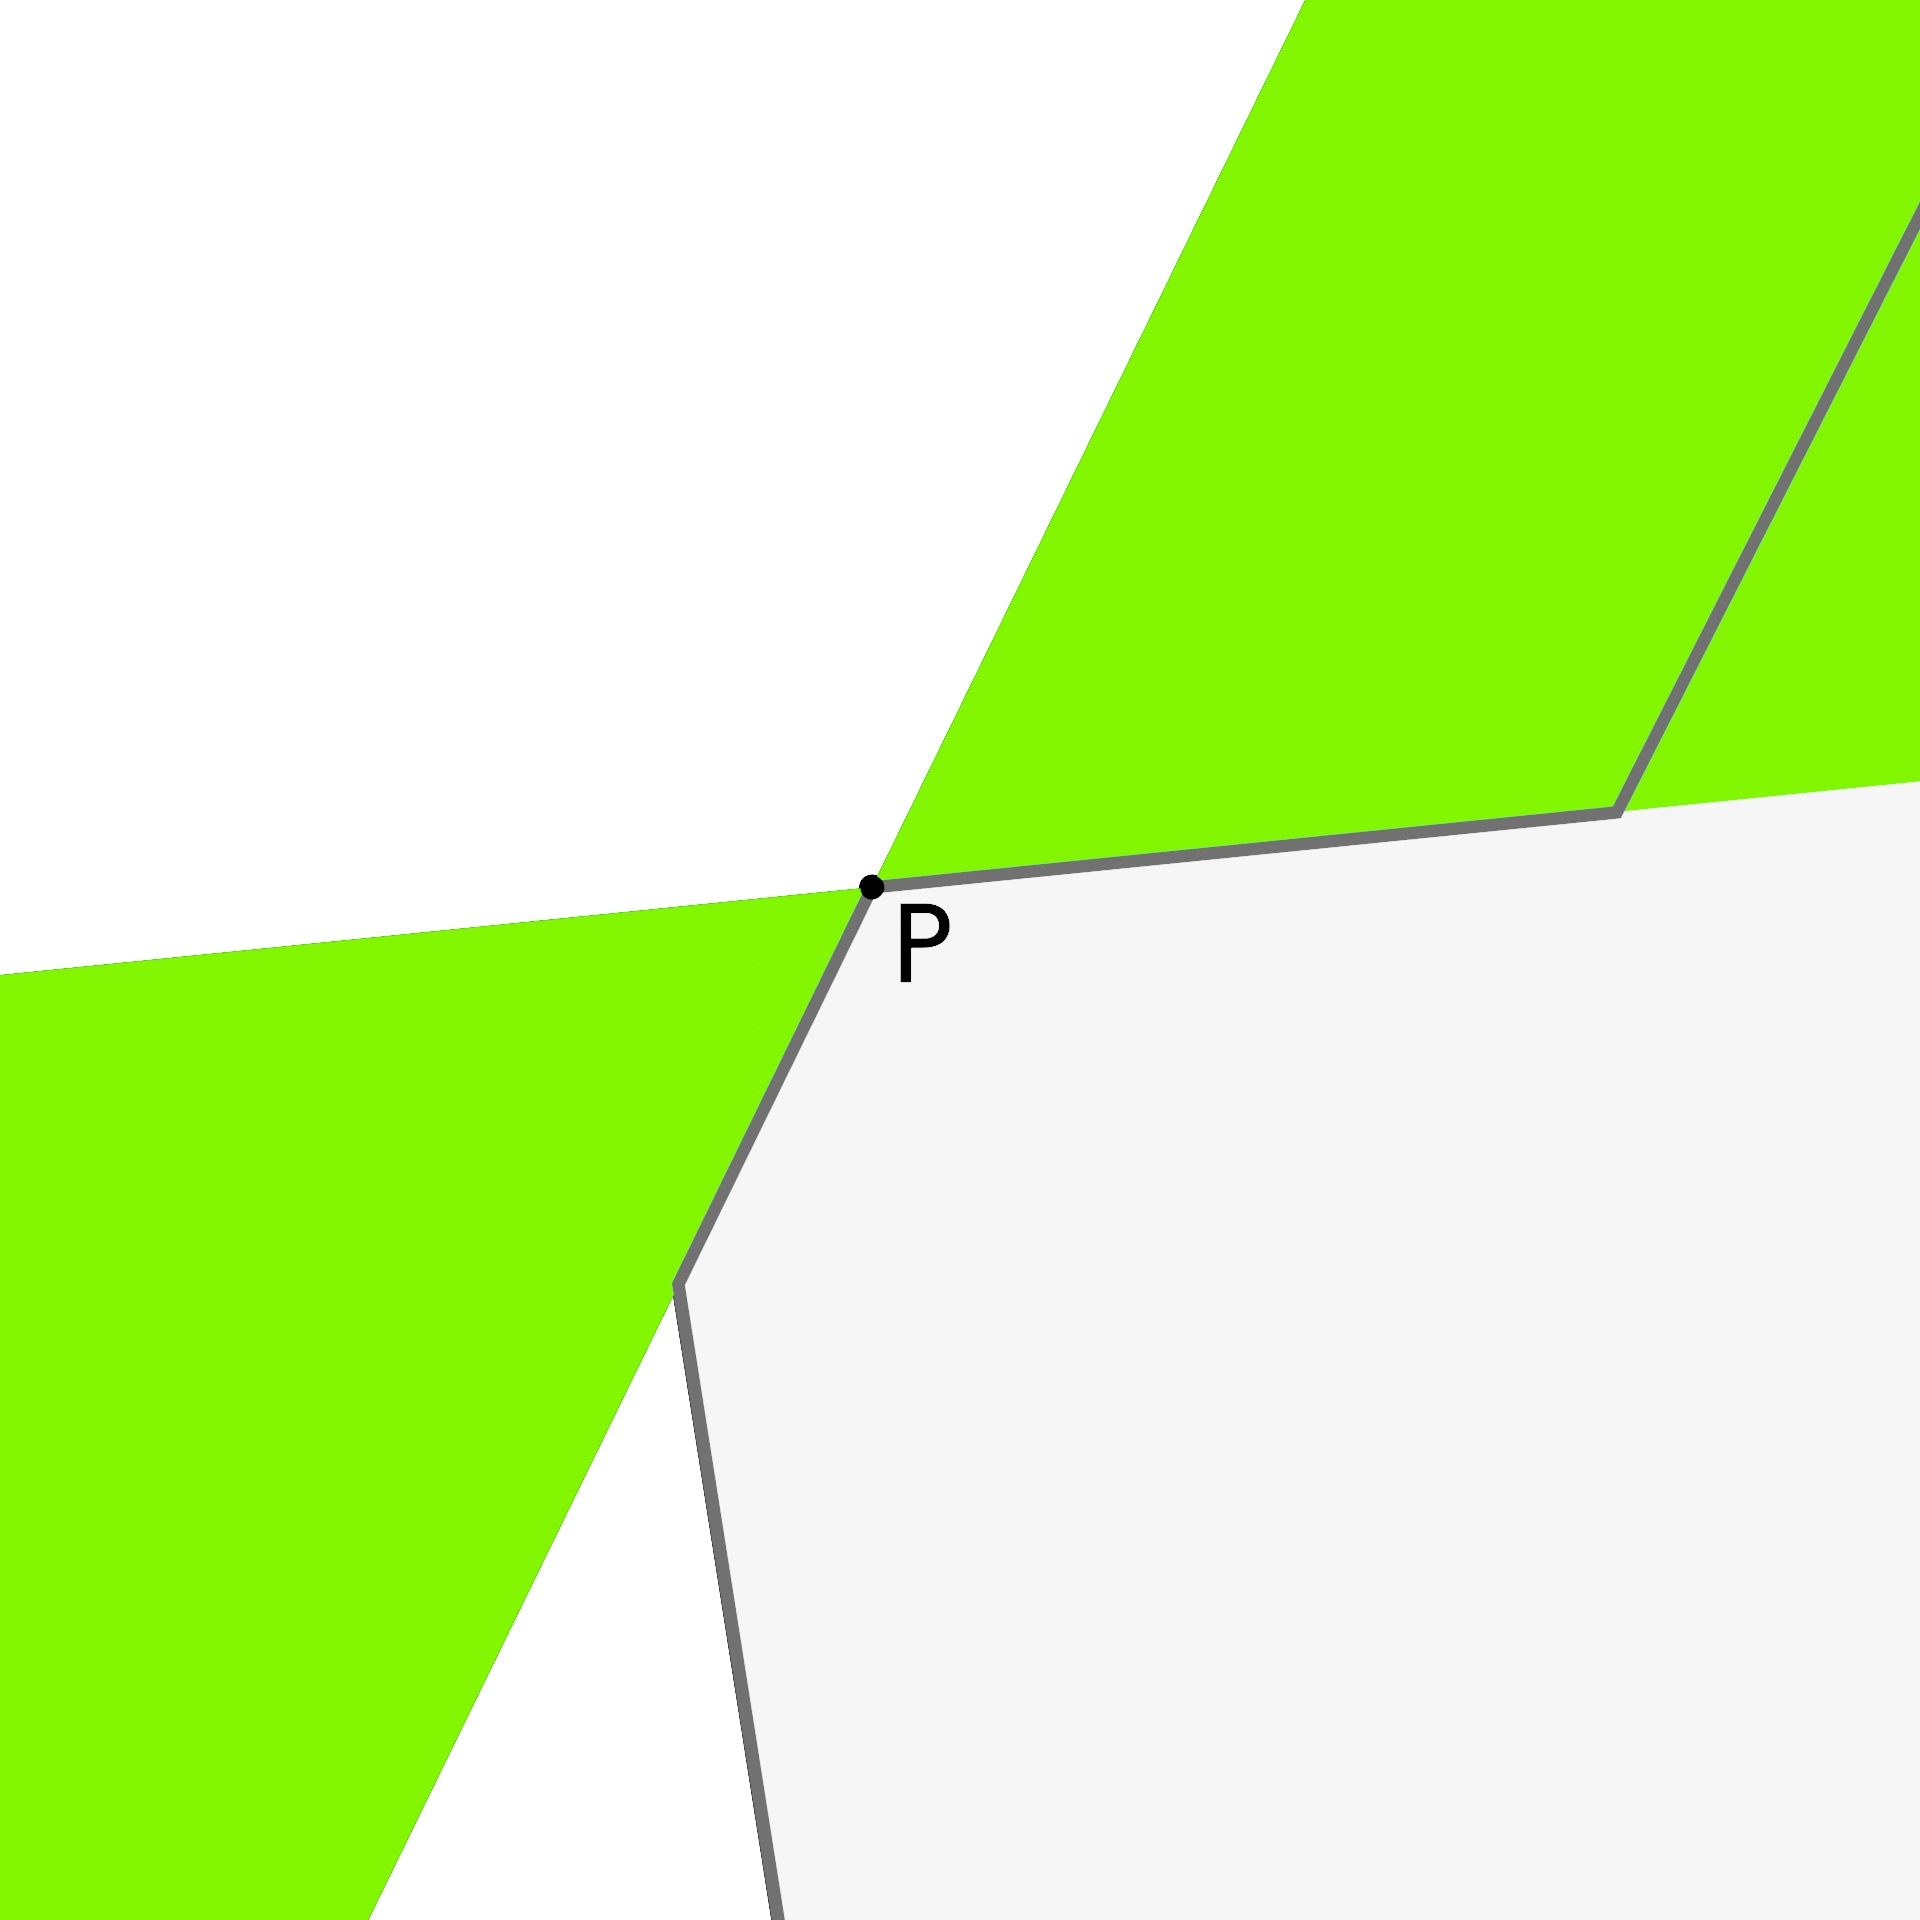
\includegraphics[scale=0.08]{Poly}}
\captionof{figure}{BetweenNeighbours}
\end{minipage}

Um das durchgehen unendlich dünner Wege zu verhindern, speichere ich die hinzugefügten/entfernten Kanten, errechne die Strecke die sie auf der Strecke zum aktuellem Punkt einnehmen, und errechne die Überschneidungen der linken und rechten Seite.

Um nun ein reduzierten Sichtbarkeitsgraphen zu generieren muss dieser Algorithmus nun nur noch für alle Punkte ausgeführt werden.

Mit dem Sichtbarkeitsgraphen fertig genreriere ich nun eine Heuristik mit Dijkstras Algorithmus, jedoch generiere ich diese nur bis allen Endpunkten (Enden der 30\degree\ Strecken, auf dem Buspfad) von Dijkstra besucht wurden (/an der Spitze der Priotitätsliste waren).

Da Dijkstra's Algorithmus nicht immer alle Knoten besucht, muss der Sichtbarkeitsgraph auch nicht vollständig generiert werden. Um dies auszunutzen berechne ich das Sichtbarkeitspolygon nur für Punkte die Dijkstra besucht.

Sobald die Heuristik fertig generiert ist, errechne mit dieser die optimale Strecke zu allen Endpunkten und die Zeit die Lisa braucht um diese abzulaufen, und die Zeit die der Bus braucht, um dorthin zu kommen. Damit errechne ich die Zeit zu der Lisa losgehen muss für alle diese Wege, vergleiche diese und nehme den Weg mit der spätesten Startezeit. Dieser Weg ist der optimale Weg, und somit das Ergebnis.

\section{Beispiele}
%TODO

\section{Code}


\end{document}